% Human-in-the-loop oversight as four expressions of one move, layered on the permission model — Ch26.
% Standalone TikZ; compiled by `book-scaffold build-figures` via pdflatex -> pdftocairo -> SVG.
% Base layer: the permission MODEL (Always / Ask / Never; permissions.deny) — labeled Vol-1 guardrails.
% On top, four expressions of the one move: (1) approval gate, (2) plan mode, (3) calibration,
% (4) escalation in automation. The vertical "workflow on model" relation is shown by a thick arrow.
\documentclass[tikz,border=4mm]{standalone}
\usepackage{tikz}
\usetikzlibrary{positioning, arrows.meta, calc}

\begin{document}
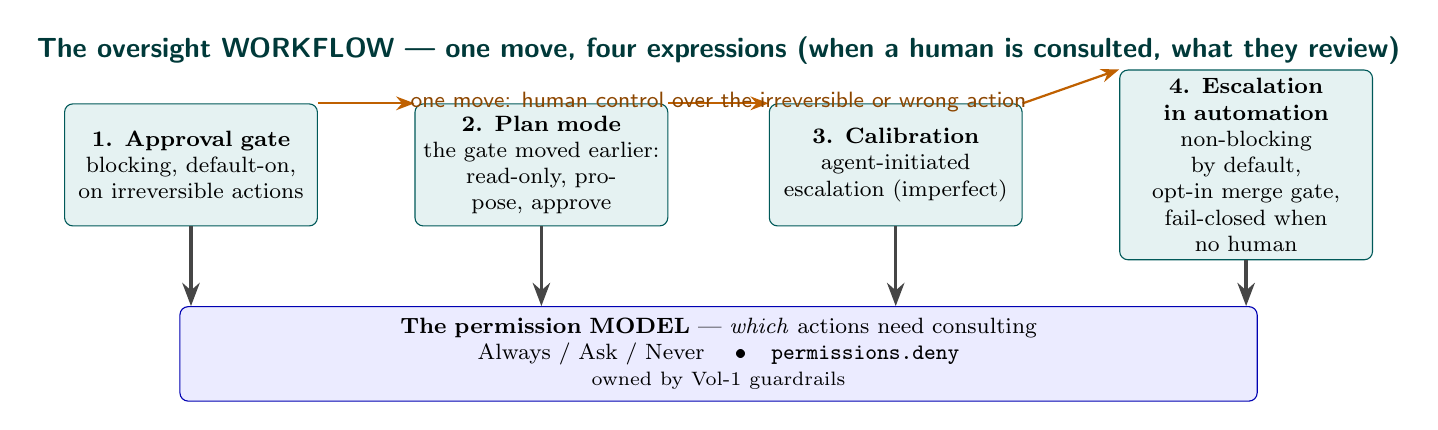
\begin{tikzpicture}[
  font=\sffamily,
  surface/.style={draw=teal!70!black, fill=teal!10, rounded corners=3pt, align=center,
    text width=3.0cm, minimum height=1.55cm, inner sep=3pt, font=\footnotesize},
  base/.style={draw=blue!70!black, fill=blue!8, rounded corners=3pt, align=center,
    text width=13.4cm, minimum height=1.2cm, inner sep=4pt, font=\footnotesize},
  flow/.style={-Stealth, very thick, draw=gray!55!black},
  lever/.style={-Stealth, thick, draw=orange!75!black}
]

% --- base layer: the permission MODEL (Vol-1 guardrails) ---
\node[base] (model) at (6.7,0)
  {\textbf{The permission MODEL} --- \emph{which} actions need consulting\\
   Always / Ask / Never \quad\textbullet\quad \texttt{permissions.deny}\\
   {\scriptsize owned by Vol-1 guardrails}};

% --- four oversight expressions, layered on top ---
\node[surface] (e1) at (0,2.4)
  {\textbf{1. Approval gate}\\blocking, default-on,\\on irreversible actions};
\node[surface] (e2) at (4.45,2.4)
  {\textbf{2. Plan mode}\\the gate moved earlier:\\read-only, propose, approve};
\node[surface] (e3) at (8.95,2.4)
  {\textbf{3. Calibration}\\agent-initiated\\escalation (imperfect)};
\node[surface] (e4) at (13.4,2.4)
  {\textbf{4. Escalation in automation}\\non-blocking by default,\\opt-in merge gate,\\fail-closed when no human};

% banner over the four expressions
\node[font=\sffamily\bfseries, text=teal!45!black] at (6.7,3.85)
  {The oversight WORKFLOW --- one move, four expressions (\emph{when} a human is consulted, \emph{what} they review)};

% --- workflow-on-model: each expression rides on the permission model ---
\draw[flow] (e1.south) -- (e1.south |- model.north);
\draw[flow] (e2.south) -- (e2.south |- model.north);
\draw[flow] (e3.south) -- (e3.south |- model.north);
\draw[flow] (e4.south) -- (e4.south |- model.north);

% the single move that runs through all four
\draw[lever] (e1.north east) -- (e2.north west);
\draw[lever] (e2.north east) -- (e3.north west);
\draw[lever] (e3.north east) -- (e4.north west);
\node[font=\sffamily\footnotesize, text=orange!55!black] at (6.7,3.2)
  {one move: human control over the irreversible or wrong action};

\end{tikzpicture}
\end{document}
